% /chapters/3-deep-computations/04-classifying.tex

\section{Classifying deep computations}\label{sec:classification}

\subsection{NIP, Rosenthal compacta, and deep computations}

This is the main section of the chapter.
We use topology of function spaces to obtain a new hierarchy of complexity classes for deep computations.
The main topological tool is Todorčević's trichotomy for Rosenthal compacta~\cite{Todorcevic_1999_CompactSubsetsBaire}. 
Our inspiration is the work of Glasner and Megrelishvili on tame semigropus in topological dynamics~\cite{glasner2022tame}.

Theorem~\ref{thm:nip-baire1def} below is the cornerstone of the section;
it establishes a powerful link between deep computations and Rosenthal compacta.
It extends the results of~\cite{alva2024approximability} from the setting of continuous deep computations to the more general (and realistic) setting of deep computations of the first Baire class.
Informally, Theorem~\ref{thm:nip-baire1def} states that if $\mathcal{P}$ and $\Delta\subseteq\Gamma$ are countable, 
then the space of deep computations generated by $\Delta$ is a Rosenthal compactum (when restricted to shards) if and only if $\Delta$ satisfies the NIP feature by feature.
Furthermore, Theorem~\ref{thm:nip-baire1def} shows that every deep computation generated by $\Delta$ is a sequential limit (rather than an abstract ultrafilter limit) of computations in $\Delta$.

\begin{theorem}\label{thm:nip-baire1def}
    Let $(L,\mathcal{P},\Gamma)$ be a compositional computation structure (Definition~\ref{def:CCS}) satisfying the Extensibility Axiom with $\mathcal{P}$ countable.
    Let $R$ be an exhaustive collection of sizers, and suppose that $\Delta\subseteq\Gamma$ is $R$-confined.
    Then the following conditions are equivalent:

    \begin{enumerate}[(i)]
        \item $\overline{\tilde\Delta\restriction_{\mathcal{L}[r_\bullet]}}\subseteq \mathrm{B}_1(\mathcal{L}[r_\bullet],\mathcal{L}[r_\bullet])$ for all $r_\bullet\in R$;
        \item $\pi_P\circ \Delta\restriction_{L[r_\bullet]}$ satisfies the NIP for all $P\in\mathcal{P}$ and $r_\bullet\in R$; that is, for all $P\in\mathcal{P}$, $r_\bullet\in R$, $a<b$, $\{\gamma_n\}_{n\in\mathbb{N}}\subseteq\Delta$ there are finite disjoint $E,F\subseteq\mathbb{N}$ such that
        \[L[r_\bullet]\cap\bigcap_{n\in E}(\pi_P\circ\gamma_n)^{-1}(-\infty,a]\cap\bigcap_{n\in F}(\pi_P\circ\gamma_n)^{-1}[b,\infty)=\emptyset.\]
    \end{enumerate}

    Furthermore, if any (hence all) of the preceding conditions hold, then every deep computation $f\in\overline{\Delta}$ can be extended to a Baire-1 function on shards: there is $\tilde f\colon\mathcal{L}_{\sh}\to \mathcal{L}_{\sh}$ such that $\tilde f\restriction_{\mathcal{L}[r_\bullet]}\in \mathrm{B}_1(\mathcal{L}[r_\bullet],\mathcal{L}[r_\bullet])$ for all $r_{\bullet}\in R$.
    In particular, on each shard, every deep computation is the pointwise limit of a countable sequence of computations.
\end{theorem}

\begin{proof}
    Since $\mathcal{P}$ is countable, $\mathcal{L}[r_\bullet]\subseteq\mathbb{R}^\mathcal{P}$ is Polish.
    The Extensibility Axiom implies that $\pi_P\circ \tilde\Delta\restriction_{\mathcal{L}[r_\bullet]}$ is a pointwise bounded set of continuous functions for all $P\in\mathcal{P}$.
    Hence, Theorem~\ref{thm:Generalized-BFT} and Lemma \ref{lem:NIP-and-closure} prove the equivalence of (i) and (ii).
    If (i) holds and $f\in\overline{\Delta}$, then we can write as an ultralimit of computations in $\Delta$, say  $f=\mathcal{U}{\rm lim}_i \gamma_i$.
    Define $\tilde f:=\mathcal{U}{\rm lim}_i \tilde\gamma_i$.
    Then, for all $r_\bullet\in R$ we have $\tilde f\restriction_{\mathcal{L}[r_\bullet]}\in\overline{\tilde\Delta\restriction_{\mathcal{L}[r_\bullet]}}\subseteq \mathrm{B}_1(\mathcal{L}[r_\bullet],\mathcal{L}[r_\bullet])$.
    The assertion that every deep computation is a pointwise limit of a countable sequence of computations follows from the fact that for a Polish space $X$, every compact subset of $\mathrm{B}_1(X)$ is Fréchet-Urysohn (that is, a space where any point in the closure of a set $A$ is the limit of a sequence of points in $A$; see Theorem 3F in \cite{BFT_1978_PCompactBaire} or Theorem 4.1 in \cite{debs2013rosenthal}).
\end{proof}

\subsection{The Todorčević trichotomy, and levels of NIP and PAC learnability}\label{sec:trichotomy}
Recall that a topological space $X$ is \emph{hereditarily separable} if every subspace is separable, and that $X$ is \emph{first countable} if every point in $X$ has a countable local basis.
Every separable metrizable space is hereditarily separable, and R.
Pol proved that every hereditarily separable Rosenthal compactum is first countable (see section 10 of \cite{debs2013rosenthal}).
This suggests the following definition:

\begin{definition}
    Let $(L,\mathcal{P},\Gamma)$ be a CCS satisfying the Extensibility Axiom and $R$ be an exhaustive collection of sizers.
Let $\Delta\subseteq\Gamma$ be an $R$-confined countable set of computations satisfying the NIP on shards and features (condition (ii) in Theorem \ref{thm:nip-baire1def}).
We say that $\Delta$ is:
    \begin{enumerate}[(i)]
        \item
        $\NIP_1$ if $\overline{\tilde\Delta\restriction_{\mathcal{L}[r_\bullet]}}$ is first countable for every $r_\bullet\in R$;
        \item
        $\NIP_2$ if $\overline{\tilde\Delta\restriction_{\mathcal{L}[r_\bullet]}}$ is hereditarily separable for every $r_\bullet\in R$;
        \item
        $\NIP_3$ if $\overline{\tilde\Delta\restriction_{\mathcal{L}[r_\bullet]}}$ is metrizable for every $r_\bullet\in R$.
    \end{enumerate}
\end{definition}

Observe that $\NIP_3 \Rightarrow \NIP_2\Rightarrow \NIP_1\Rightarrow \NIP$.
We now present examples of separable and non-separable examples Rosenthal compacta that show that implications are strict.
These examples are due to Todorčević \cite{Todorcevic_1999_CompactSubsetsBaire}.

\begin{example}\label{exa:Rosenthal-compacta}
\hfill
\begin{enumerate}
    \item \emph{Alexandroff compactification of a discrete space of size continuum}.
    The subset $\mathcal{A} = \mathcal{D}_{\mathfrak{c}}\cup\{\mathbf{0}\} \subseteq \mathrm{B}_1(2^{\mathbb{N}})$ in~§\ref{sec:extended-alexandroff} is the Alexandroff (one-point) compactification of the continuum-size discrete set~$\mathcal{D}_{\mathfrak{c}} = \{\bbar{x}: x\in 2^{\mathbb{N}}\}$.
    Hence, $\mathcal{A}$ is a Rosenthal compactum that is not hereditarily separable (and therefore not first countable).
    In particular, $\mathcal{A}$ is not separable.

    \item \emph{Extended Alexandroff compactification}.
    The Alexandroff compactification $\mathcal{A}$ of $\mathcal{D}_{\mathfrak{c}}$ above can be embedded into a separable compactum of $\mathrm{B}_1(2^{\mathbb{N}})$ by adding a countable set $\mathcal{A}^{\complement}$ of new points that “soften” neighbourhoods in~$\mathcal{A}$, yielding the extended compactification $\mathcal{A}_{\mathrm{E}} = \mathcal{A}\cup \mathcal{A}^{\complement}$ of~§\ref{sec:extended-alexandroff}.
    However, the separable Rosenthal compactum $\mathcal{A}_{\mathrm{E}}$ is not first countable.
    It is an example of a CCS that is NIP but not $\NIP_1$.

    \item \emph{Split Cantor}.
    The split Cantor set $\cancel{C}$ is a separable Rosenthal compactum that is $\NIP_2$ but not $\NIP_3$; it is hereditarily separable, but it is not metrizable.
    The set of all finite-precision classifiers is countable dense in~$\cancel{C}$.

    \item \emph{Alexandroff Duplicate}.
    Let $K$ be any compact metric space.
    Construct the space $X = K\sqcup \mathrm{C}(K)$, i.e., the disjoint union of $K$ and the space $\mathrm{C}(K)$ of real-valued continuous functions on $K$ with the Banach topology of uniform convergence (supremum-norm topology).
    Clearly, $X$ is Polish.
    For each $a\in K$, define $g_a^0,g_a^1\colon X\to\mathbb{R}$ as follows:
    \[
    g_a^0(x)=\begin{cases}
        0, & \text{if }x\in K\\
        x(a), & \text{if }x\in \mathrm{C}(K);
    \end{cases}
    \]
    \[
	g_a^1(x)=\begin{cases}
        \Brack{a = x}, & \text{if }x\in K;\\
        x(a), & \text{if }x\in \mathrm{C}(K).
    \end{cases}
    \]
    Let $\mathrm{D}(K)=\{g_a^0:a\in K\}\cup\{g_a^1:a\in K\}$.
Observe that all points $g_a^1$ are isolated and that open neighbourhoods of $g_{a_0}^0$ are of the form $\{g_a^i:a\in U,i\in\{0,1\}\}\setminus\{g_a^1:a\in F\}$ where $U\subseteq K$ is an open neighbourhood of $a_0$ and $F\subseteq K$ is a finite set.

Another way to present this space is as the space $K\times\{0,1\}$ with the identifications
$(a,0)\mapsto g_a^0$ and $(a,1)\mapsto g_a^1$ and the
basic open neighbourhoods are given asabove.
We can also embed $\mathrm{D}(K)$ into the product $A(K)\times K$ by identifying $(a,0)\mapsto (\mathbf{0},a)$ and $(a,1)\mapsto (\delta_a,a)$.

Notice that $\mathrm{D}(K)$ is a first countable Rosenthal compactum.
It is not separable if $K$ is uncountable; thus, we typically study the interesting case when $K=2^\mathbb{N}$.

As with the Alexandroff compactification $A(2^{\mathbb{N}})$, we can make the space $\mathrm{D}(2^{\mathbb{N}})$ separable  by ``softening'' the neighbourhoods of each point through the addition of a countable set.
For example, the closure of the set $\{(v_s,s^\frown 0^\infty):s\in 2^{<\mathbb{N}}\}\subseteq \hat{A}(2^{\mathbb{N}})\times 2^{\mathbb{N}}$ is $\{(\mathbf{0},a):a\in 2^{\mathbb{N}}\}\cup \{(\delta_a,a):a\in 2^{\mathbb{N}}\}\cup\{(v_s,s^\frown 0^\infty):s\in 2^{<\mathbb{N}}\}$, where $\{(\mathbf{0},a):a\in 2^{\mathbb{N}}\}\cup \{(\delta_a,a):a\in 2^{\mathbb{N}}\}$ is homeomorphic to $\mathrm{D}(2^{\mathbb{N}})$.

    \item \emph{Extended Alexandroff Duplicate of the Split Cantor}.
    For each finite binary sequence $t\in 2^{<\mathbb{N}}$, let $a_t\in 2^\mathbb{N}$ be the sequence starting with $t$ and ending with $0$'s and let $b_t\in 2^\mathbb{N}$ be the sequence starting with $t$ and ending with $1$'s.
    Define $h_t\colon 2^\mathbb{N}\to\mathbb{R}$ by
    \[
	h_t(x)=\begin{cases}
        0, & \text{if }x<a_t;\\
        1/2, & \text{if }a_t\leq x \leq b_t;\\
        1, & \text{if }b_t<x.
    \end{cases}
    \]
    Let $\hat{D}(S(2^\mathbb{N}))$ be the pointwise closure of the set $\{h_t:t\in 2^{<\mathbb{N}}\}$.
    The identification $h_t\mapsto (v_t,f_{t^\frown 0^\infty}^+)$ lifts to a homeomorphism between $\hat{D}(S(2^\mathbb{N}))$ and the subspace of $\hat{A}(2^\mathbb{N})\times S(2^\mathbb{N})$ consisting of $(\mathbf{0},f_a^+)$, $(\mathbf{0},f_a^-)$, $(\delta_a,f_a^+)$ and $(v_t,f_{t^\frown 0^\infty}^+)$ for $a\in 2^{\mathbb{N}}$ and $t\in 2^{<\mathbb{N}}$ (see 4.3.7 in \cite{argyros2008rosenthal}).
Hence, $\hat{D}(S(2^\mathbb{N}))$ is a separable first countable Rosenthal compactum that is not hereditarily separable.
In fact, it contains an uncountable discrete subspace.
\end{enumerate}

\end{example}

\begin{theorem}[Todorčević's Trichotomy, \cite{Todorcevic_1999_CompactSubsetsBaire}, {\cite[Theorem~3]{argyros2008rosenthal}}]\label{thm:Todorcevic-trichotomy}
    Let $K$ be a separable Rosenthal Compactum.
    \begin{enumerate}[(i)] 
        \item 
        If $K$ is hereditarily separable but non-metrizable, then $S(2^\mathbb{N})$ embeds into $K$.
        \item 
        If $K$ is first countable but not hereditarily separable, then either $\mathrm{D}(2^\mathbb{N})$ or $\hat{D}(S(2^\mathbb{N}))$ embeds into $K$.
        \item
         If $K$ is not first countable, then $A(2^\mathbb{N})$ embeds into $K$.
    \end{enumerate}
\end{theorem}

We thus have the following classification for separable Rosenthal compacta:

\begin{figure}[htbp]
    \centering
    %figures/separable-compacta.tex

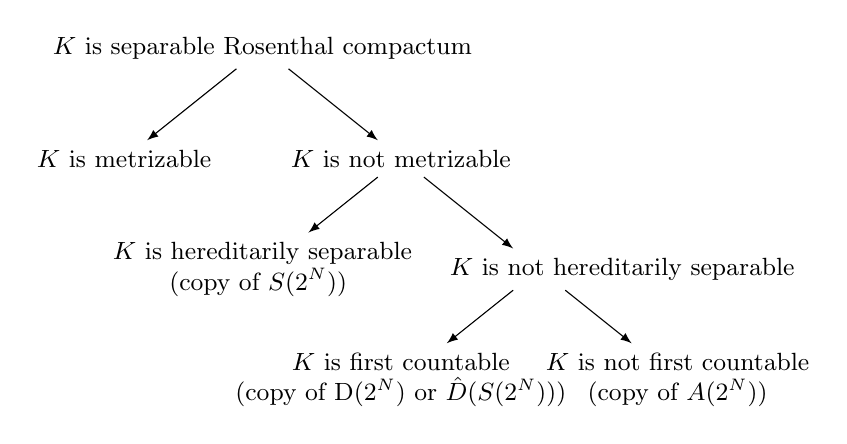
\begin{tikzpicture}[grow=down,
    sibling distance=10em,
    level distance=4em,
    edge from parent/.style={draw,-latex},
    every node/.style={font=\small,align=center}]

\node {$K$ is separable Rosenthal compactum}
    child {node {$K$ is metrizable}}
    child {node {$K$ is not metrizable}
    child {node {$K$ is hereditarily separable \\ (copy of $S(2^\mathbb{N})$) \hspace{2cm}}}
    child {node {\hspace{2cm} $K$ is not hereditarily separable}
    child {node {$K$ is first countable \\ (copy of $\mathrm{D}(2^\mathbb{N})$ or $\hat{D}(S(2^\mathbb{N}))$)}}
    child {node {$K$ is not first countable \\ (copy of $A(2^\mathbb{N})$)}}}};
\end{tikzpicture}
    \caption{Classification of separable Rosenthal compacta.}
    \label{fig:separable_compacta}
\end{figure}

Todorčević's Trichotomy suggests that in order to distinguish the classes $\NIP_i$, the examples in \ref{exa:Rosenthal-compacta} are essential.
The following examples show that the levels $\NIP_i$ ($i=1,2,3$) may be distinguished by the topological complexity of deep computations.

\begin{example}\label{exa:NIP-levels}
\hfill
\begin{enumerate}
    \item Let $(L,\mathcal{P},\Gamma)$ be the computation of square root (example \ref{exa:square-roots-compute} with $\Delta=\Gamma$).
    We saw that $\overline{\tilde{\Delta}}=\tilde{\Delta}\cup\{\tilde{f}\}\subseteq \mathrm{B}_1(\mathcal{L},\mathcal{L})$.
    This corresponds to the Alexandroff compactification of a countable discrete set, which is metrizable. Hence, $\Delta$ is $\NIP_3$ but it is not stable, in the sense that $\overline{\tilde{\Delta}}\not\subseteq \mathrm{C}(\mathcal{L},\mathcal{L})$.

    \item Let $(L,\mathcal{P},\Gamma)$ be the finite precision threshold classifiers (Section~\ref{sec:Cantor-classifiers}) with $\Delta=\{\phi_w:w\in 2^{<\mathbb{N}}\}\cup\{\mathbf{0^\infty},\mathbf{1^\infty}\}$.
    We saw that $\overline{\Delta}$ is homeomorphic to the Split Cantor space $S(2^\mathbb{N})$ (Example \ref{exa:Rosenthal-compacta}-(3)), which is hereditarily separable but not metrizable.
    Hence, $\Delta$ is $\NIP_2$ but not $\NIP_3$.

    \item Let $(L,\mathcal{P},\Gamma)$ be the CCS given by $L=2^{\mathbb{N}}$, $\mathcal{P}=\{P_n:n\in\mathbb{N}\}$ and $\Gamma$ is the semigroup generated by $\Delta=\{\gamma_t:t\in 2^{<\mathbb{N}}\}$, where $P_n\colon 2^\mathbb{N}\to\{0,1\}$ is the projection map $P_n(x)=x(n)$ and $\gamma_t\colon L\to L$ is given by
    \[
	\gamma_t(x)=\begin{cases}
        0^\infty, & \text{if }x<_{\text{lex}}t^\frown0^\infty;\\
        (01)^\infty, & \text{if }t^\frown0^\infty\leq_{\text{lex}} x \leq_{\text{lex}} t^\frown1^\infty;\\
        1^\infty, & \text{if }t^\frown1^\infty<_{\text{lex}}x.
    \end{cases}
    \]
    where $(01)^\infty$ denotes the sequence of alternating bits: $010101\cdots$. 
    As in the other examples, it is not difficult to see that $(L,\mathcal{P},\Gamma)$ satisfies the Extensibility Axiom.
    For example, the condition $t^\frown0^\infty\leq_{\text{lex}} x \leq_{\text{lex}} t^\frown1^\infty$ is equivalent to $x$ extending $t$.
    Observe that the set of deep computations is homeomorphic to $\hat{D}(S(2^{\mathbb{N}}))$ (see Example~\ref{exa:Rosenthal-compacta}-(5)).
    Hence, $\Delta$  is $\NIP_1$ but not $\NIP_2$.

    \item Let $(L,\mathcal{P},\Gamma)$ be the finite precision prefix test (Section~\ref{sec:prefix-test}) with $\Delta=\{\psi_w:w\in 2^{<\mathbb{N}}\}$.
    We saw that $\overline{\tilde{\Delta}}$ is homeomorphic to the Extended Alexandroff compactification $\hat{A}(2^\mathbb{N})$ (Example \ref{exa:Rosenthal-compacta}-(3)), which is separable but not first countable.
    Hence, $\Delta$ is NIP but not $\NIP_1$.
\end{enumerate}
\end{example}

The definitions provided here for $\NIP_i$ ($i=1,2,3$) are topological.
This raises the following question:

\begin{question}
    Is there a non-topological characterization for $\NIP_i$, $i=1,2,3$?
\end{question}

\subsection{The Argyros-Dodos-Kanellopoulos heptachotomy, and approximability of deep computation by minimal classes}\label{sec:heptachotomy}

In the three separable cases given in \ref{exa:Rosenthal-compacta}, namely, $\hat{A}(2^\mathbb{N})$, $S(2^\mathbb{N})$ and $\hat{D}(S(2^\mathbb{N}))$, the countable dense subsets are indexed by the binary tree $2^{<\mathbb{N}}$.
This choice of index is useful because our emphasis is computational.
Real numbers can be represented as infinite binary sequences, i.e., infinite branches of the binary tree $2^{\mathbb{N}}$, and
we approximate real numbers with elements in $2^{<\mathbb{N}}$, i.e., finite bitstrings.

\begin{definition}
    Let $X$ be a Polish space.

    \begin{enumerate}
        \item If $I$ is countable and $\{f_i:i\in I\}\subseteq\mathbb{R}^X$, $\{g_i:i\in I\}\subseteq\mathbb{R}^X$ are two pointwise families by $I$, we say that $\{f_i:i\in\ I\}$ and $\{g_i:i\in I\}$ are \emph{equivalent} if and only if the map $f_i\mapsto g_i$ is extended to a homeomorphism from $\overline{\{f_i:i\in I\}}$ to $\overline{\{g_i:i\in I\}}$.
        \item If $\{f_t:t\in 2^{<\mathbb{N}}\}$ is a pointwise bounded family, we say that $\{f_t:t\in 2^{<\mathbb{N}}\}$ is \emph{minimal} if and only if for every dyadic subtree $\{s_t:t\in 2^{<\mathbb{N}}\}$ of $2^{<\mathbb{N}}$, $\{f_{s_t}:t\in 2^{<\mathbb{N}}\}$ is equivalent to $\{f_t:t\in 2^{<\mathbb{N}}\}$.
    \end{enumerate}
\end{definition}

One of the main results in \cite{argyros2008rosenthal} is that, up to equivalence, there are seven minimal families of Rosenthal compacta and that for every relatively compact $\{f_t:t\in 2^{<\mathbb{N}}\}\subseteq \mathrm{B}_1(X)$ there is a dyadic subtree $\{s_t:t\in 2^{<\mathbb{N}}\}$ such that $\{f_{s_t}:t\in 2^{<\mathbb{N}}\}$ is equivalent to one of the minimal families.
We shall describe the seven minimal families next.
We follow the same notation as in \cite{argyros2008rosenthal}.
For any node $t\in 2^{<\mathbb{N}}$, we denote by $t^\frown 0^{\infty}$ ($t^\frown 1^{\infty}$) the infinite binary sequence starting with $t$ and continuing with all $0$'s (respectively, all $1$'s).
Fix a regular dyadic subtree $R=\{s_t:t\in 2^{<\mathbb{N}}\}$ of $2^{<\mathbb{N}}$ (i.e., a dyadic subtree such that every level of $R$ is contained in a level of $2^{<\mathbb{N}}$) with the property that for all $s,s'\in R$, we have $s^\frown 0^{\infty}\neq s'^\frown 0^\infty$ and $s^\frown 1^{\infty}\neq s'^\frown 1^\infty$.
Given $t\in 2^{<\mathbb{N}}$, let $v_t$ be the characteristic function of the set $\{x\in 2^\mathbb{N}:x \text{ extends } t\}$.
Let $<$ be the lexicographic order in $2^\mathbb{N}$.
Given $a\in 2^{\mathbb{N}}$, let $f^+_a\colon 2^{\mathbb{N}}\to\{0,1\}$ be the characteristic function of $\{x\in 2^{\mathbb{N}}:a\leq x\}$ and let $f^-_a\colon 2^{\mathbb{N}}\to\{0,1\}$ be the characteristic function of $\{x\in 2^{\mathbb{N}}:a>x\}$.
Given two maps $f,g\colon 2^{\mathbb{N}}\to\mathbb{R}$ we denote by $(f,g)\colon 2^{\mathbb{N}}\sqcup 2^{\mathbb{N}}\to\mathbb{R}$ the function which is $f$ on the first copy of $2^{\mathbb{N}}$ and $g$ on the second copy of $2^{\mathbb{N}}$.

\begin{enumerate}
    \item $D_1=\{\frac{1}{|t|+1}v_t:t\in 2^{<\mathbb{N}}\}$.
    This is discrete in $\overline{D_1}=A(2^{\mathbb{N}})$.
    \item $D_2=\{s_t^\frown 0^{\infty}:t\in 2^{<\mathbb{N}}\}$.
    This is discrete in $\overline{D_2}=2^{\leq N}$.
    \item $D_3=\{f^+_{s_t^\frown 0^\infty}:t\in 2^{<\mathbb{N}}\}$.
    This is discrete in $\overline{D_3}=S(2^{\mathbb{N}})$.
    \item $D_4=\{f^-_{s_t^\frown 1^\infty}:t\in 2^{<\mathbb{N}}\}$.
    This is discrete in $\overline{D_4}=S(2^{\mathbb{N}})$.
    \item $D_5=\{v_t:t\in 2^{<\mathbb{N}}\}$.
    This is discrete in $\overline{D_5}=\hat{A}(2^{\mathbb{N}})$.
    \item $D_6=\{(v_{s_t},s_t^\frown 0^\infty):t\in 2^{<\mathbb{N}}\}$.
    This is discrete in $\overline{D_6}=\hat{D}(2^{\mathbb{N}})$.
    \item $D_7=\{(v_{s_t},x^+_{s_t^\frown 0^\infty}):t\in 2^{<\mathbb{N}}\}$.
    This is discrete in $\overline{D_7}=\hat{D}(S(2^{\mathbb{N}}))$.
\end{enumerate}

\begin{theorem}[Heptachotomy of minimal families, Theorem 2 in \cite{argyros2008rosenthal}]
    Let $X$ be Polish.
    For every relatively compact $\{f_{t}:t\in 2^{<\mathbb{N}}\}\subseteq \mathrm{B}_1(X)$, there exists $i=1,2,\dots, 7$ and a regular dyadic subtree $\{s_t:t\in 2^{<\mathbb{N}}\}$ of $2^{<\mathbb{N}}$ such that $\{f_{s_t}:t\in 2^{<\mathbb{N}}\}$ is equivalent to $D_i$.
    Moreover, the families $D_i$ are minimal and mutually non-equivalent.
\end{theorem}

The implication of this result for deep computations is the following: 
for any countable set of computations $\Delta$ satisfying the NIP (for some CCS $(L,\mathcal{P},\Gamma)$), we can always find a countable discrete set of deep computations that approximates all the other deep computations.
For example: in the finite precision prefix test example (subsection \ref{sec:prefix-test}), the prefix test computations (family $D_5$) approximate all other deep computations.
However, note that this discrete set $D_i$ may not consist of continuous functions (i.e., they will not be computable in general).
For example, functions in $D_3$ are not continuous.